\chapter{Program do sterowania pomiarami charakterystyk laserów półprzewodnikowych z wykorzystaniem sprzętu Thorlabs}
\section{Wstęp}
W ramach pracy inżynierskiej zostały stworzone programy do sterowania pomiarami charakterystyk laserów.
Program został napisany w dwóch wersjach: skryptowej oraz okienkowej. Podstawą działania programów są następujące klasy:
\begin{itemize}
\item $\mathtt{device.py}$ --- główna klasa, zawiera funkcje: do sprawdzania dostępnych urządzeń,
funkcje zwracającą instancje danego urządzenia, co umażliwa sterowanie danym urządzeniami.
\item $\mathtt{IODevice.py}$ --- klasa do operacji wejścia-wyjścia na programowalnych urządzeniach pomiarowych. Jest to
uniwersalna klasa, która może być użyta do dowolnego urządzenia zgodnego ze standardem SCPI. Do jej obsługi wymagane jest
podanie ścieżki do urządzenia.
\item $\mathtt{LDC4005.py}$ --- klasa zawierająca funkcje od obsługi zasilacza diód laserowych Thorlabs LDC4005. Implementacja
funkcji oparta jest na poleceniach SCPI dla LDC4005~\cite{Ldc_book_prog}.
\item $\mathtt{PM100.py}$ --- klasa zawierająca funkcje do obsługi detektora mocy Thorlabs PM100. Implementacja
funkcji oparta jest na poleceniach SCPI dla PM100~\cite{Pm100_book}.
\end{itemize}
\section{Krótki opisz najważniejszych klas}
W tym podrozdziale przedstawię stworzone kody programów do sterowania pomiarami charakterystyk laserów półprzewodnikowych.
 W zaprezentowanych kodach przedstawiam tylko najważniejsze funkcje, aby ułatwić czytelność (pełny kod jest dołączony do pracy).

Pierwszy listing 3.1 przedstawia klasę $\mathtt{IODevice.py}$ do operacji  wejścia-wyjścia na urządzeniach programowalnych.
Jest to podstawowa klasa, która następnie używana jest w klasach do sterowania zasilaczem
diod laserowych - $\mathtt{LDC4005.py}$ (listing 3.2) oraz do sterowania miernikiem mocy - $\mathtt{PM100.py}$ (listing 3.3).
Ostatni kod (listing 3.4) pokazuje przykładowy skrypt w języku Python 3, którym można wykonać pomiar charakterystyki lasera.
\newpage
\lstinputlisting[language=Python, firstline=0, lastline=20]{IODevice.py}
\lstinputlisting[language=Python, firstline=0, lastline=20]{PM100.py}
\lstinputlisting[language=Python, firstline=0, lastline=29]{LDC4005.py}
Skrypt przedstawiony na listingu 3.4 w wierszach 1-3 importuje potrzebne moduły, ważne, aby moduły $\mathtt{LDC4005.py}$ oraz $\mathtt{PM100.py}$
znajdowały się w tym samym folderze co $\mathtt{measure.py}$.
W wierszu 6 deklamujemy tablice 20 elementów o wartościach prądu od 0 do 0.02 \,A. Następnie w wierszach 8-10 deklarujemy tablice do przechowywania danych, które zostaną zmierzone. W liniach 13-14 tworzy instancje klasy dla zasilacza i miernika, zakładamy, że port $\mathtt{/dev/usbtmc0}$ odpowiada zasilaczowi ldc4005, a port $\mathtt{/dev/usbtmc1}$ odpowiada miernikowi mocy PM100.
Następnie w wierszy 20 ustawiany prąd na zasilaczu, w 21 czytamy prąd z zasilacza, w 22 czytamy napięcie, a w 23 czytamy moc wyjściową na mierniku mocy.
Ostatnim etapem jest zapisanie danych do pliku  przedstawione w wierszach 25-26.
\lstinputlisting[language=Python, firstline=0, lastline=26]{measure.py}
\section{Wersja skryptowa programu}
Jedna z możliwością przeprowadzania pomiarów jest wykorzystanie skryptu (wraz z innymi klasami dołączony jest do pracy).
Struktura programu pokazana jest na rysunku \ref{struktura_rys_1}. Aby zainstalować wszystkie niezbedne biblioteki należy
w konsoli wywołać polecenie $\mathtt{make}$.
\begin{lstlisting}[style=Bash]
student@ubuntu:~$ make
\end{lstlisting}
Nastepnie uruchamiamy wirtualne środowisko (linia 1), które posiada wszystkie potrzebne biblioteki, następnie
przechodzimy do katologu $\mathtt{examples}$, gdzie znajduje się plik $\mathtt{measure.py}$, który należy użyć do
przeprowadzenia pomiarów:
\begin{lstlisting}[style=Bash]
student@ubuntu:~$ source venvenv/bin/activate
student@ubuntu:~$ cd examples/
\end{lstlisting}
W celu przeprawadzenia pomiarów wywolujemy skrypt $\mathtt{measure.py}$ z parametrami:
\begin{itemize}
\item nr: liczba punktów do pomiaru
\item sc: początkowa wartość prądu w mA, od którego należy rozpocząć pomiar
\item ec: wartość prądu w mA do którego przeprowadza się pomiar.
\item fn: nazwa wynikowa pliku z danymi, która będzie zapisana w katalogu $\mathtt{output}$
\end{itemize}
\begin{lstlisting}[style=Bash]
student@ubuntu:~$ python3 measure.py -nr 150 -sc 0 -ec 20
-fn dane
\end{lstlisting}
\begin{figure}
\center
  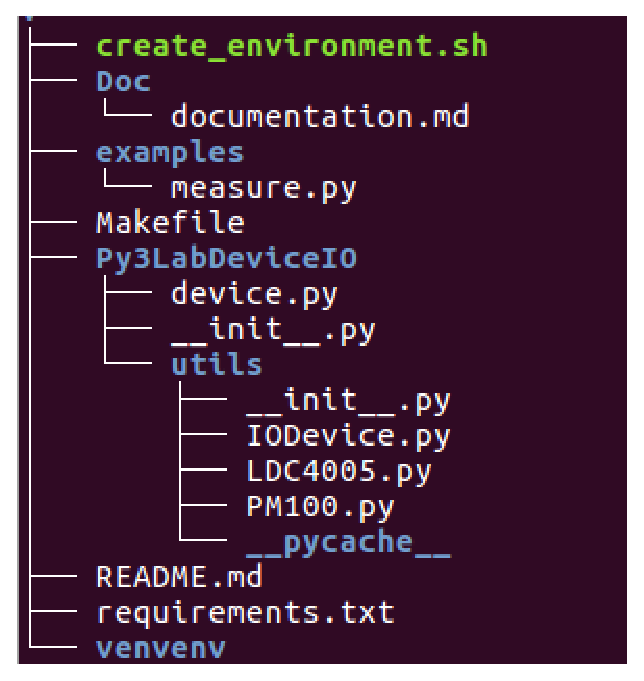
\includegraphics[scale=0.3]{tree.eps}
  \caption{Struktura programu skryptowego.}
  \label{struktura_rys_1}
\end{figure}
\section{Wersja okienkowa programu do pomiarów}
Na rysunku \ref{gui_rys} przedstawiony jest okienkowy program do wykonywania charakterystyk. Program napisany jest w języku
Python 2.7 z wykorzystaniem bibliotek PyQt5, matplotlib
\begin{figure}[h]
\center
  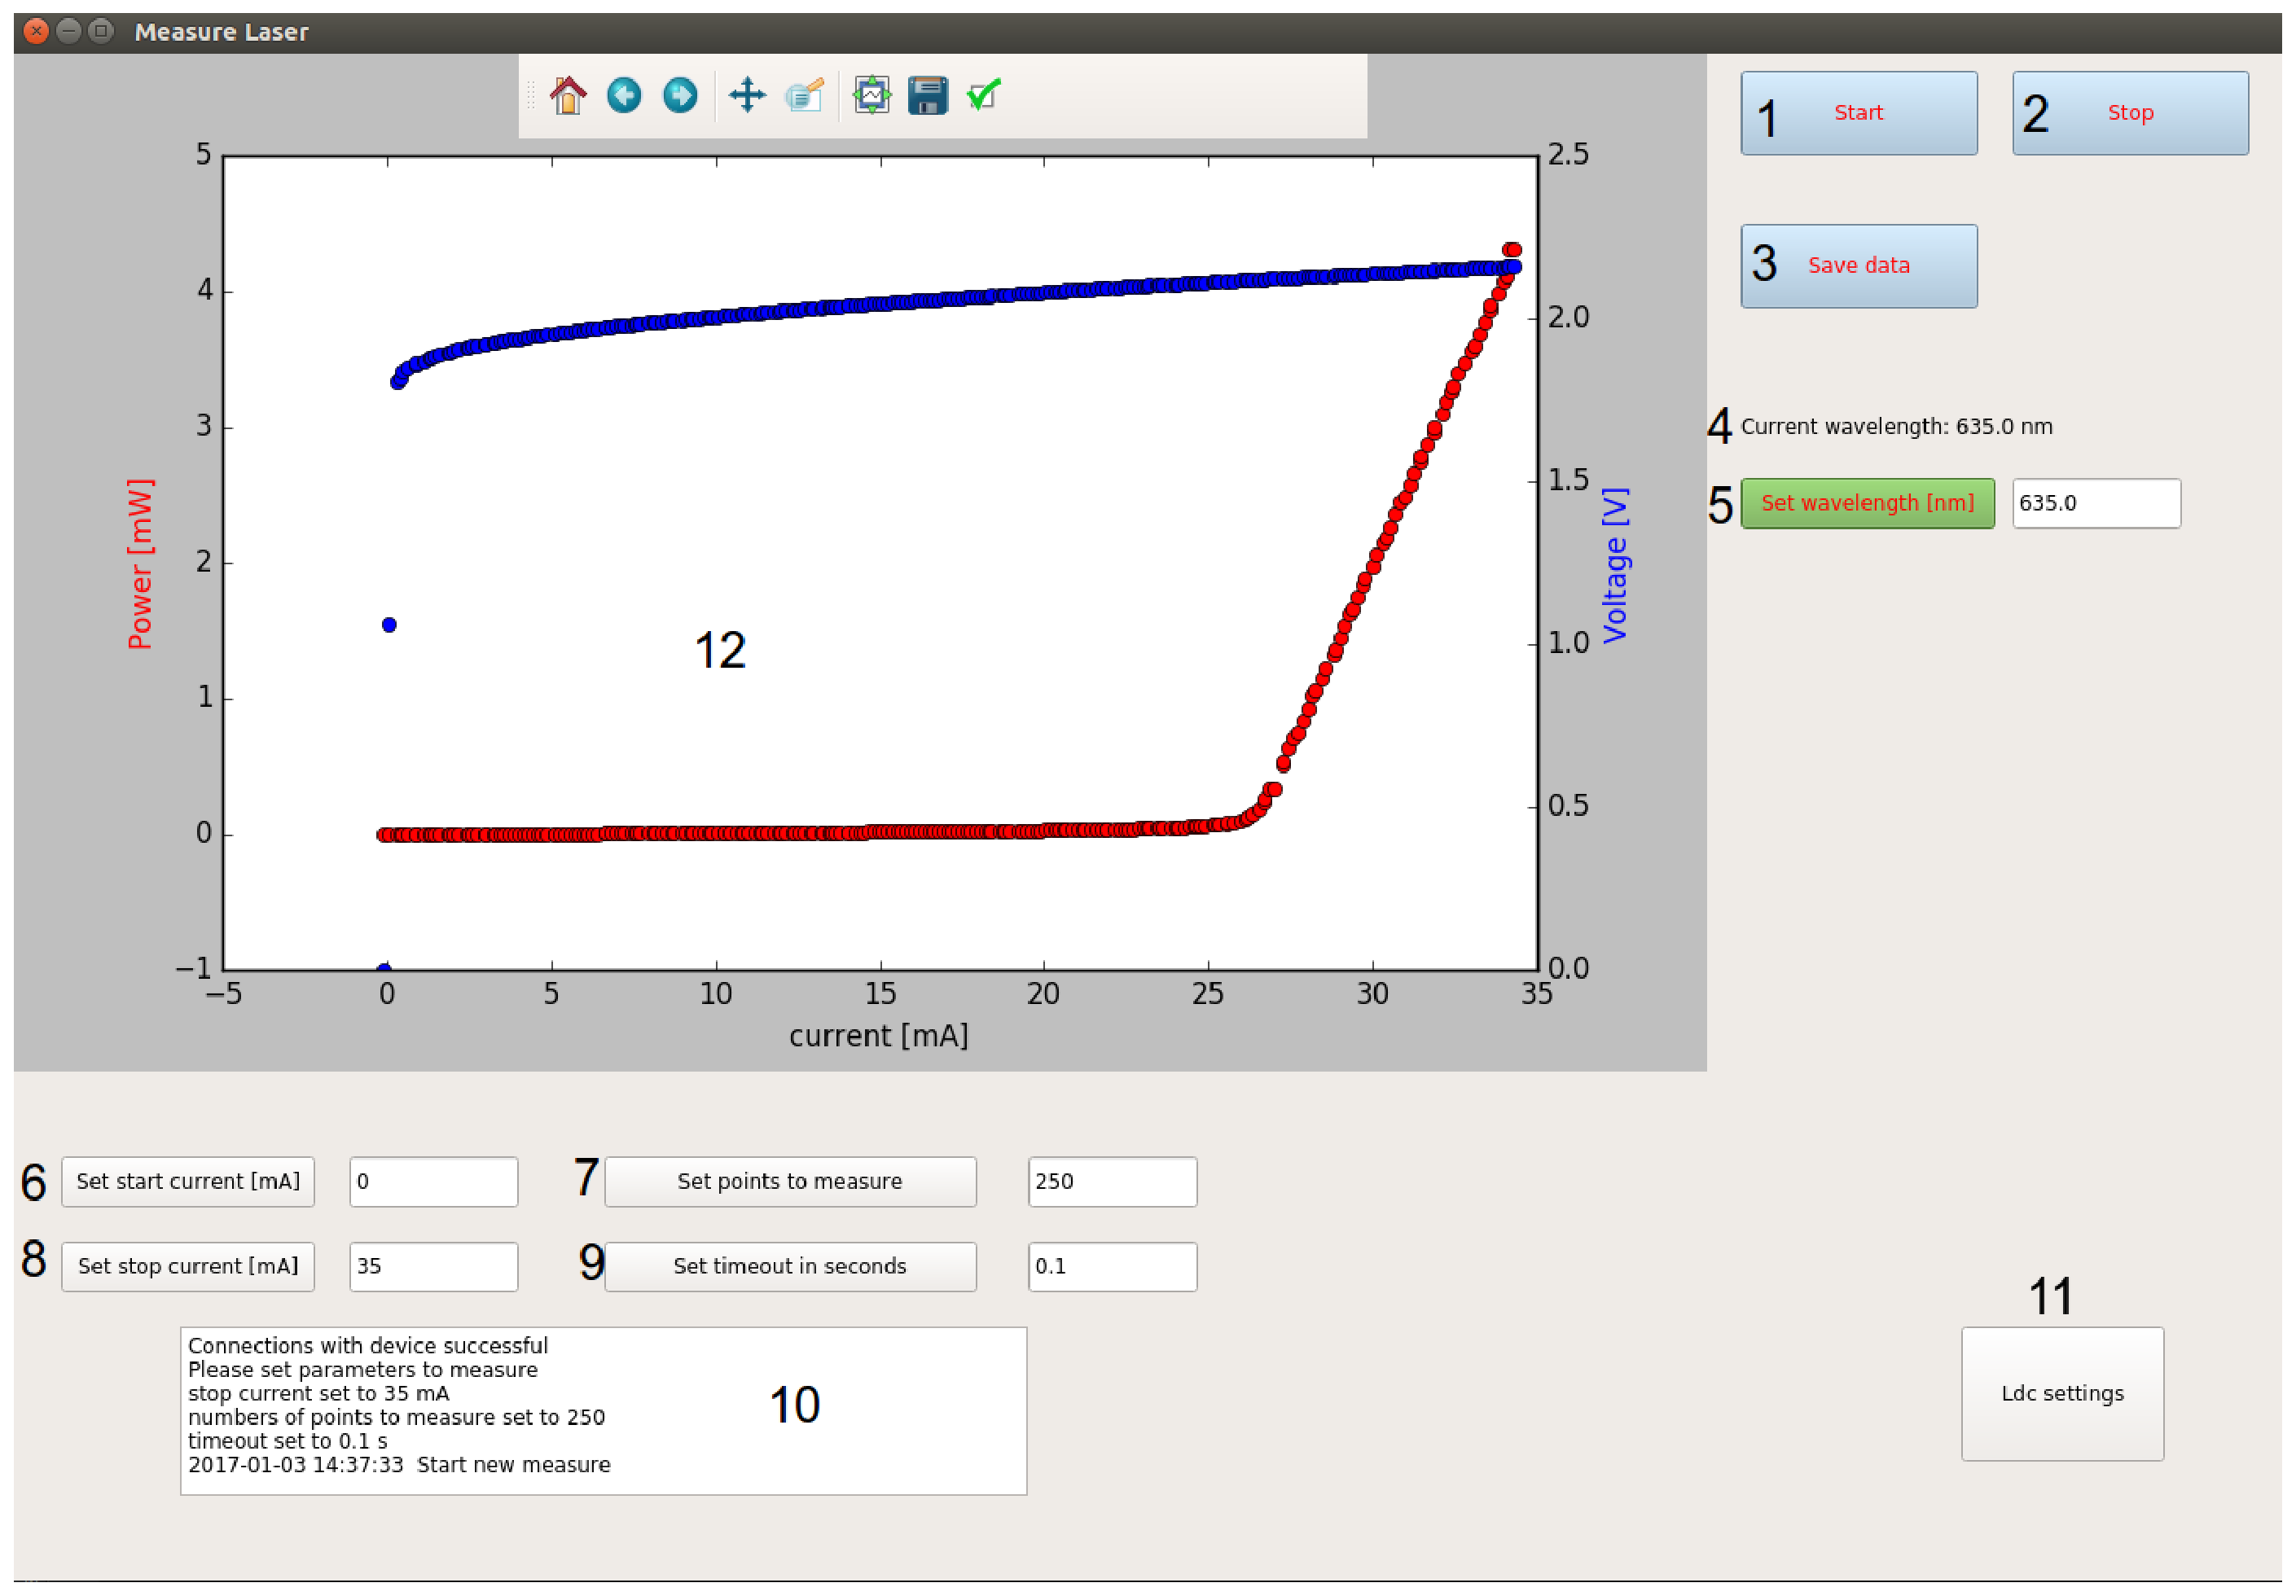
\includegraphics[scale=0.35]{gui.eps}
  \label{gui_rys}
  \caption{1 --- rozpoczecie pomiarów, 2 --- zatrzymanie pomiarów, 3 --- zapisanie danych pomiarowych, 4 --- pokazuje długość fali detektora,
   5 --- zmiana długości fali detektora 6 --- ustawia prąd początkowy do pomiarów, 7 ---  ustawia ilość punktów do pomiaru,
   8 --- ustawia prąd końcowy do pomiarów, 9 --- ustawia długość pauzy pomiędzy pomiarami, 10 --- wyświetla ważne informacje o ustawieniach,
   11 --- ustawienie zasilacza, 12 --- pokazuje charakterystykę.}
\end{figure}
\newpage
\begin{itemize}
\item Przycisk ,,Start" [1] służący do rozpoczęcia pomiarów. Po jego wciśnięciu nastąpi wykonanie charakterystyki lasera na podstawie ustawionych parametrów.
\item Przycisk ,,Stop" [2] służący do zatrzymania pomiarów. Po jego wciśnięciu nastąpi wyłączenie zasilacza.
\item Przycisk ,,Save data" [3] służący do zapisania zebranych danych. Po wciśnięciu należy wybrać ścieżkę. Zapis dokonywany jest w formacie txt.
\item Wyświetlacz długości fali wybranej na detektorze [4]. Długość fali wyświetlana jest w nanometrach.
\item Przycisk służący do zmiany długości fali na detektorze [5]. Wartość należy wprowadzić w nanometrach i zatwierdzić.
\item Przycisk ,,Set start current" [6] --- służy do wybrania prądu, od jakiego ma się zacząć pomiar w mA.
\item Przycisk ,,Set points to measure" [7] --- służy do wybrania ilości punktów do charakterystyki.
\item Przycisk ,,Set stop current" [8] --- służy do wybrania granicy prądu, do jakiego ma się odbyć pomiar w mA.
\item Przycisk ,,Set timeout in seconds" [9] --- służy do ustawienie długości pauzy między zadaniem prądu do zasilacza, a wykonaniem pomiaru.
\item Okienko informacyjne [10] --- wyświetla informacje o pomiarze.
\item Przycisk "Ldc settings" [11] --- ustawia najważniejsze parametry zasilacza diod takie jako wartość maksymalna prądu.
\item Ekran główny [12] --- pokazuje w czasie rzeczywistym zależność napięcia na laserze oraz mocy wyjściowej w funkcji
prądu wejściowego.
\end{itemize}